\documentclass{beamer}
% \usetheme{metropolis}
\usefonttheme{structuresmallcapsserif}
\usepackage{times}

\title{Linear Regression: Inference}
\author{Connor K. Brubaker}
\institute{
Department of Statistics \\
Texas A\&M University
}
\date{}

\begin{document}
\maketitle

\begin{frame}{Linear Model}
    Suppose we have data $(X_1, Y_1), \ldots, (X_n, Y_n)$. The simple linear regression model states that 
    \begin{equation*}
        Y_i = \beta_0 + \beta_1 X_i + \varepsilon_i
    \end{equation*}
    where $\varepsilon_i \sim \mathcal{N}(0, \sigma^2)$ is the error term. 
    \begin{itemize}
        \item $\beta_0$ is the intercept parameter
        \item $\beta_1$ is the slope parameter
    \end{itemize}
\end{frame}

\begin{frame}{Assumptions of the Linear Model}
    The simple linear model makes four assumptions:
    \begin{enumerate}
        \item $X$ and $Y$ are linearly related,
        \item the errors $\varepsilon_1, \ldots, \varepsilon_n$ are independent of each other,
        \item the errors $\varepsilon_1, \ldots, \varepsilon_n$ have a common variance $\sigma^2$, and 
        \item the errors $\varepsilon_1, \ldots, \varepsilon_n$ are normally distributed with a mean of $0$ and variance $\sigma^2$.
    \end{enumerate}
    For now, assume these are satisfied. We will revisit checking these assumptions (known as \textbf{model validation}) in the following lecture. 
\end{frame}

\begin{frame}{Assumptions of the Linear Model}
    \begin{center}
        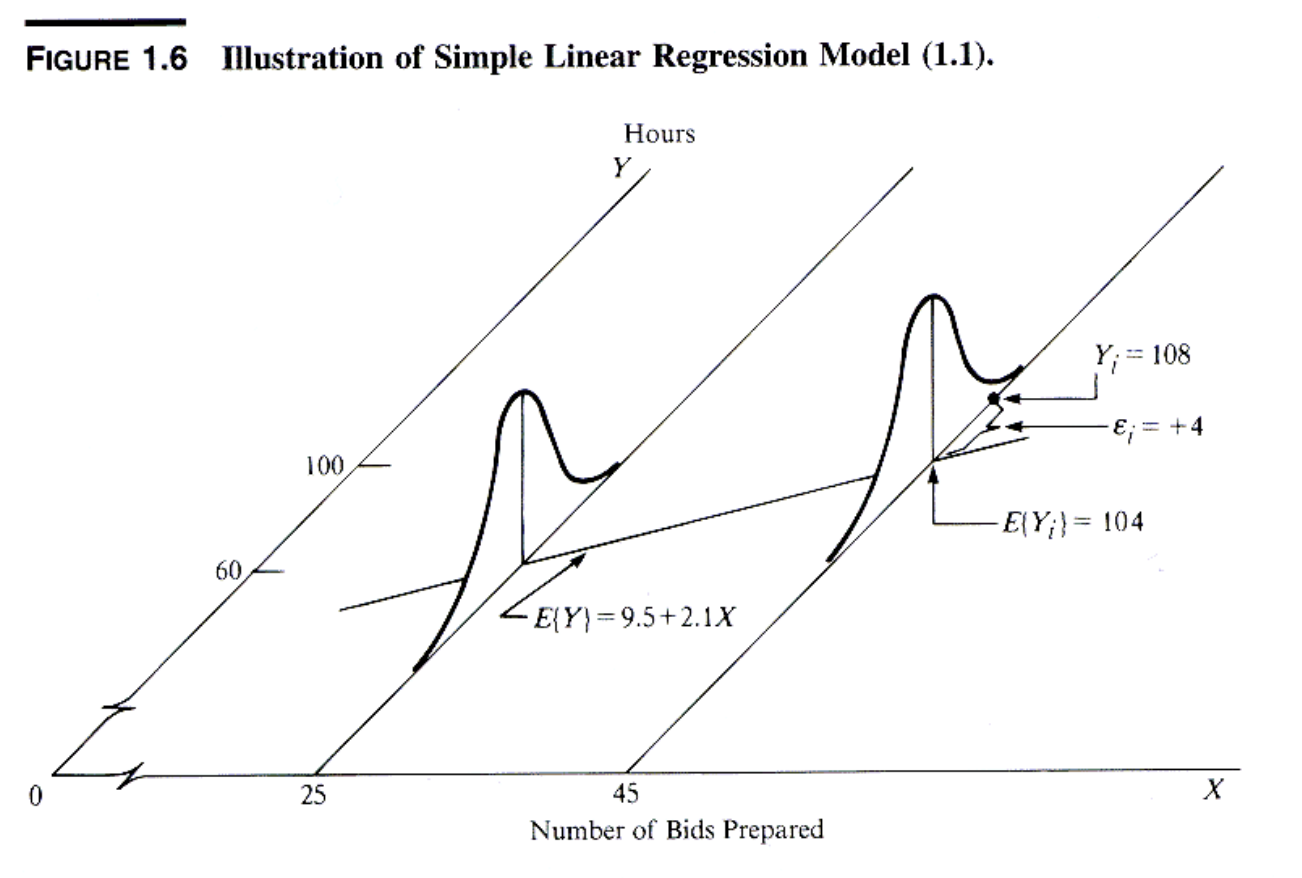
\includegraphics[width=.9\linewidth]{figures/linear_regression_normal.png}
    \end{center}
    \footnotesize 
    Source: \href{https://sphweb.bumc.bu.edu/otlt/MPH-Modules/BS/R/R5_Correlation-Regression/R5_Correlation-Regression4.html}{https://sphweb.bumc.bu.edu/otlt/MPH-Modules/BS/R/R5\_Correlation-Regression/R5\_Correlation-Regression4.html}
\end{frame}

\begin{frame}{Least Squares Estimators}
    Recall that the least squares estimators are 
    \begin{equation*}
        \hat{\beta}_1 = \frac{SXY}{SXX}\ \ \textrm{and}\ \ \hat{\beta}_0 = \bar{Y} - \hat{\beta}_1 \bar{X}.
    \end{equation*}
    where 
    \begin{equation*}
        SXY = \sum_{i=1}^n (X_i - \bar{X})(Y_i - \bar{Y})\ \ \textrm{and}\ \ SXX = \sum_{i=1}^n (X_i - \bar{X})^2.
    \end{equation*}
\end{frame}

\begin{frame}{Estimation of the Error Variance $\sigma^2$}
    Using the least squares estimates, the $i$th error is estimated with
    \begin{equation*}
        \hat{\varepsilon}_i = Y_i - \hat{Y}_i = Y_i - \hat{\beta}_0 - \hat{\beta}_1 X_i
    \end{equation*}
    The variance of the errors $\sigma^2$ is estimated using 
    \begin{equation*}
        \hat{\sigma}^2 = \frac{1}{n-1}\sum_{i=1}^n \hat{\varepsilon}_i^2 = \frac{RSS}{n-1}
    \end{equation*}
\end{frame}

\begin{frame}{Inference for the Slope Parameter $\beta_1$}
    As long as the assumptions of the simple linear model are satisfied, it can be shown that 
    \begin{equation*}
        \hat{\beta}_1 \sim \mathcal{N}\left(\beta_1, \frac{\sigma^2}{SXX}\right)
    \end{equation*}
    where $\beta_1$ is the true (unknown) slope parameter and $\sigma^2$ is the variance of the error terms. Therefore, the standard error of the slope is 
    \begin{equation*}
        \textrm{SE}(\hat{\beta}_1) = \frac{\sigma}{\sqrt{SXX}}
    \end{equation*}
    where $\sigma$ is estimated using $\hat{\sigma} = \sqrt{\hat{\sigma}^2}$. 
\end{frame}

\begin{frame}{Confidence Interval for the Slope}
    A $(1-\alpha)\times 100$\% confidence interval for $\beta_1$ is 
    \begin{equation*}
        \hat{\beta}_1 \pm t^*_{\alpha/2, n-2} \times \textrm{SE}(\hat{\beta}_1) = \hat{\beta}_1 \pm t^*_{\alpha/2, n-2} \times \frac{\hat{\sigma}}{\sqrt{SXX}}
    \end{equation*}
    The degrees of freedom is $n-2$ since we are estimating $2$ parameters (the slope and the intercept).
\end{frame}

\begin{frame}{Hypothesis Testing for the Slope}
    Often we want to test whether a significant linear relationship exists between $X$ and $Y$. If no relationship exists, then 
    \begin{equation*}
        \textrm{Cov}(X, Y) = 0
    \end{equation*}
    and consequently $\beta_1 = 0$. Therefore, we want to test the hypotheses 
    \begin{equation*}
        H_0: \beta_1 = 0\ \ \textrm{versus}\ \ H_A: \beta_1 \neq 0
    \end{equation*}
    This is the test \texttt{R} performs by default.
\end{frame}

\begin{frame}{Hypothesis Testing for the Slope}
    Let $\beta_1^{0}$ be the null value of the slope (often $0$). 

    \vspace*{1em}
    The test statistic for the hypothesis test is 
    \begin{equation*}
        T_{obs} = \frac{\hat{\beta}_1 - \beta_1^{0}}{\textrm{SE}(\hat{\beta}_1)} = \frac{\hat{\beta}_1 - \beta_1^{0}}{\hat{\sigma} / \sqrt{SXX}} \sim t_{n-2}
    \end{equation*}
    You would use the $t$ distribution with $n-2$ degrees of freedom to find critical values and determine $p$-values. 
\end{frame}

\begin{frame}{Housing Prices}
    \begin{center}
        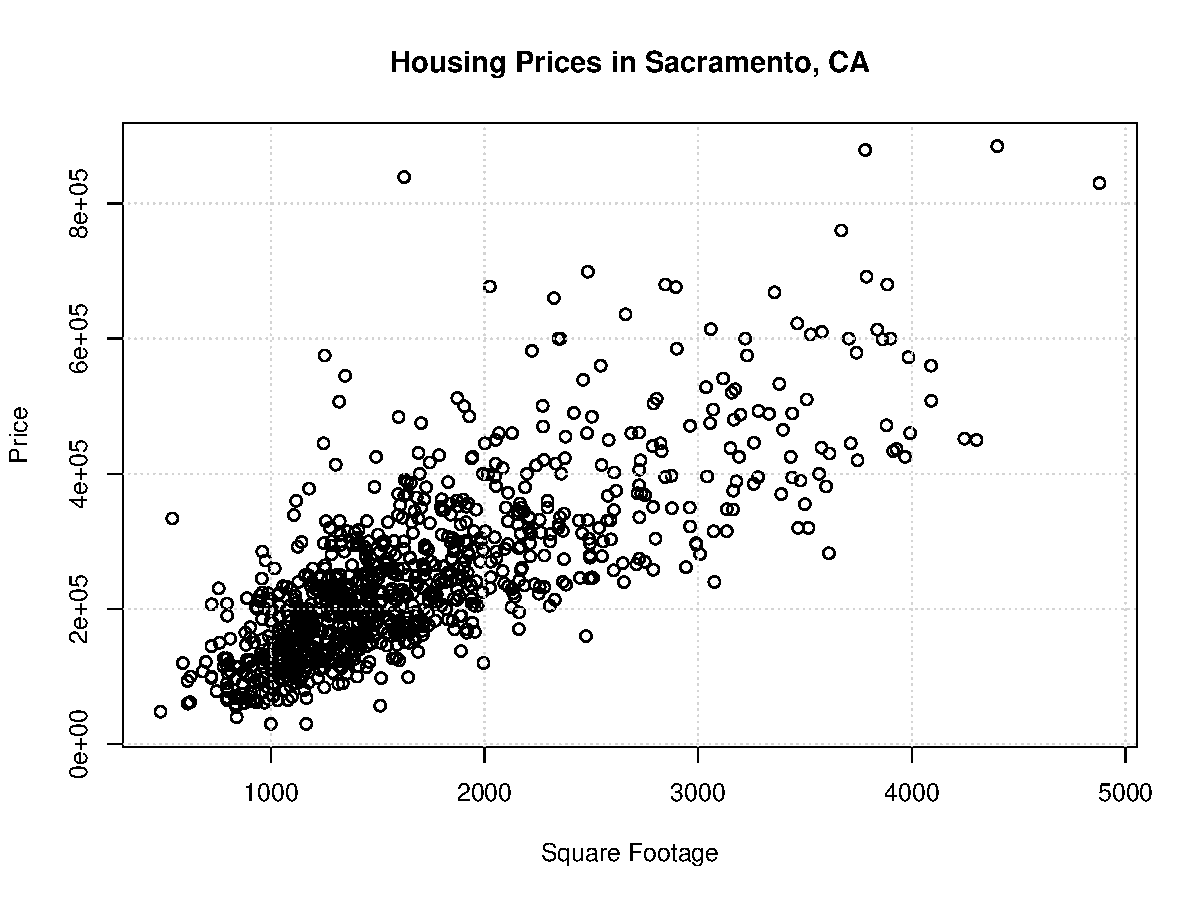
\includegraphics[width=.85\linewidth]{figures/sacramento.pdf}
    \end{center}
\end{frame}

\begin{frame}{Reading \texttt{R} Output}
    \begin{center}
        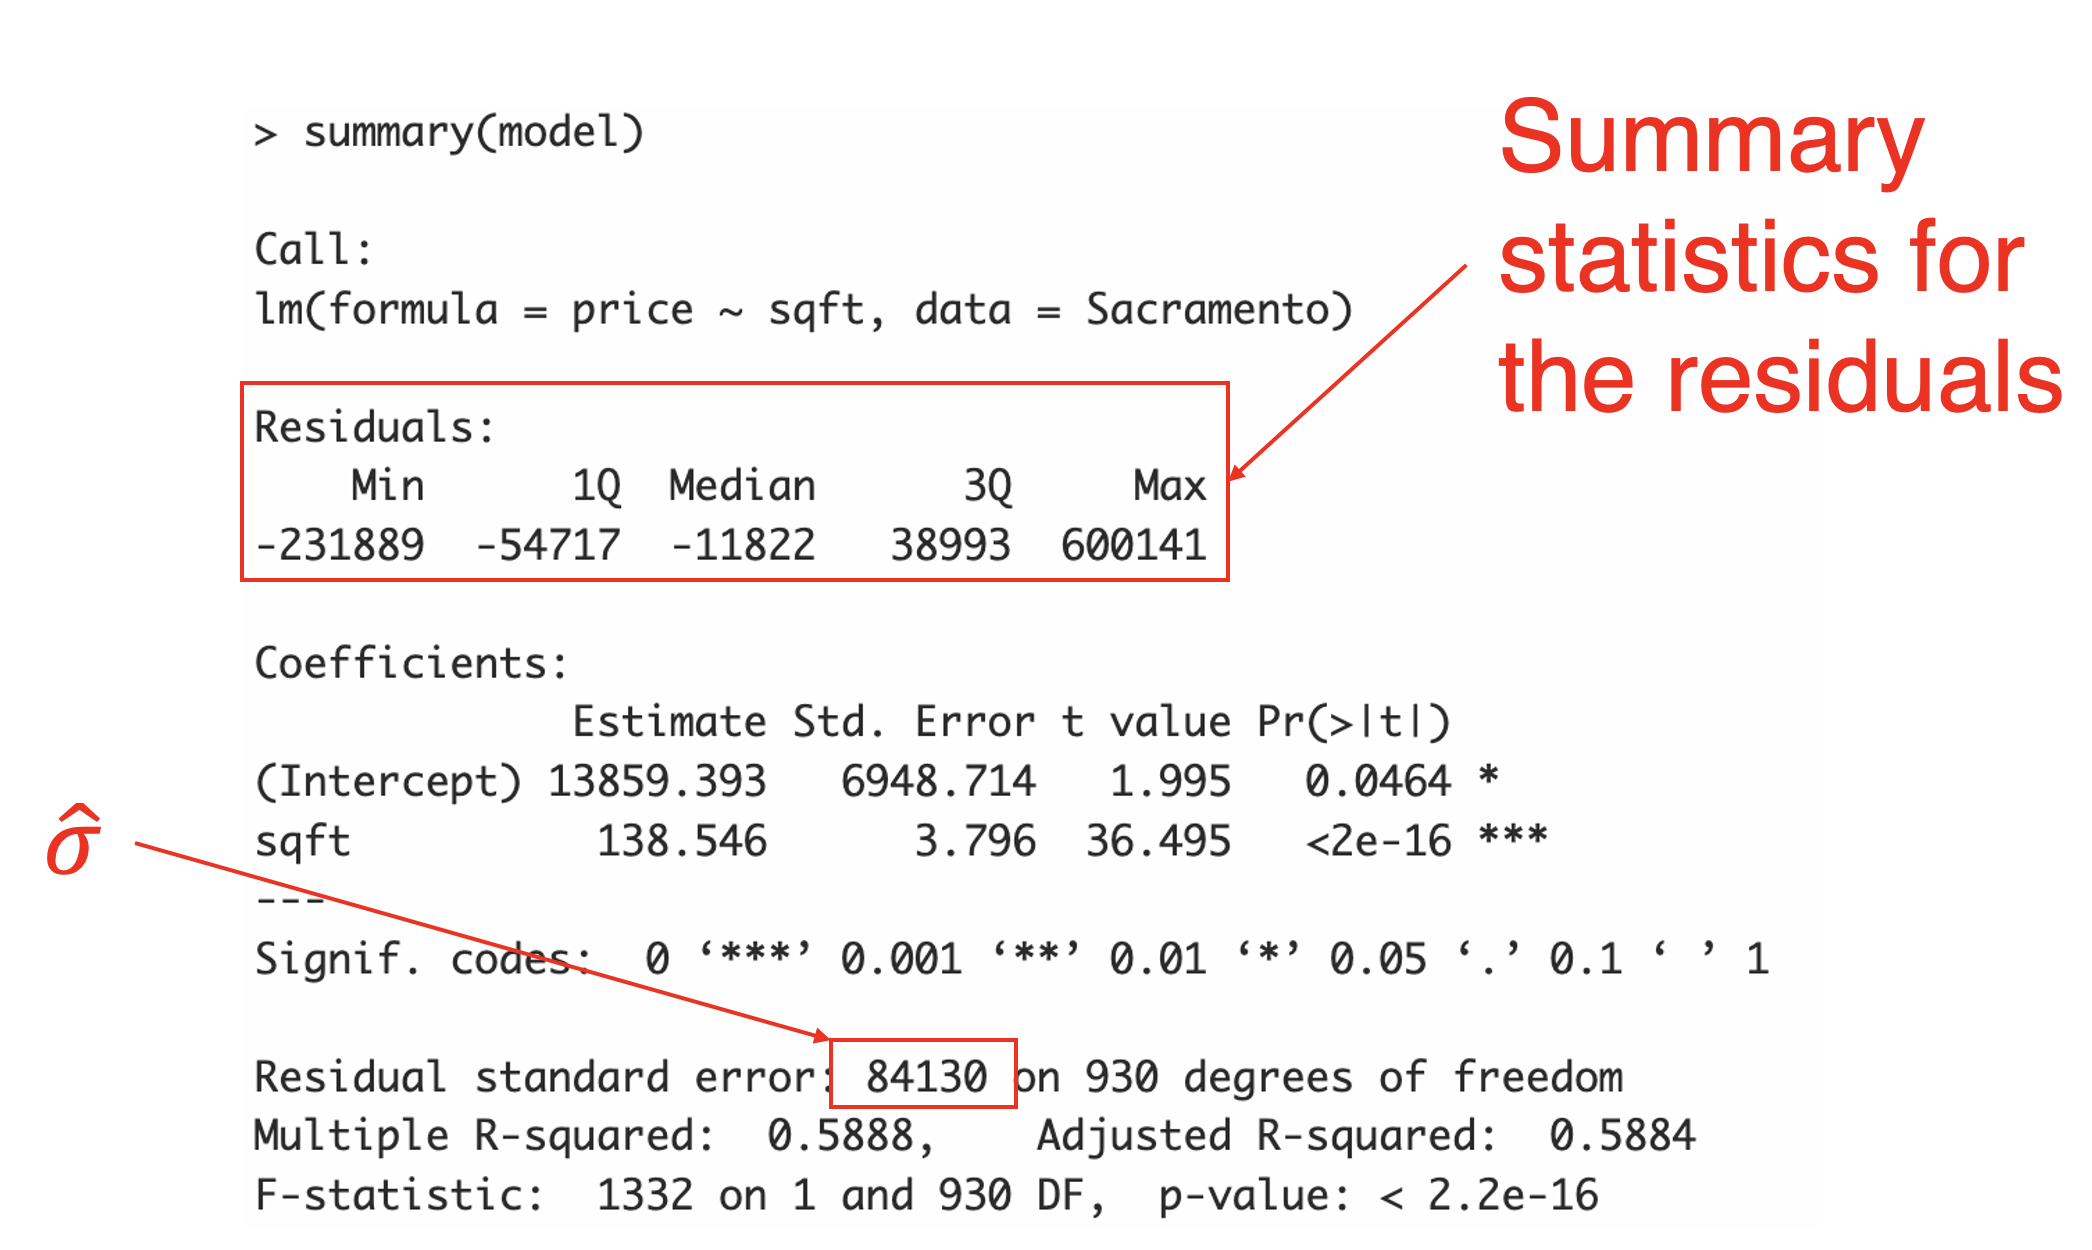
\includegraphics[width=\linewidth]{figures/resid.png}
    \end{center}
\end{frame}

\begin{frame}{Reading \texttt{R} Output}
    \begin{center}
        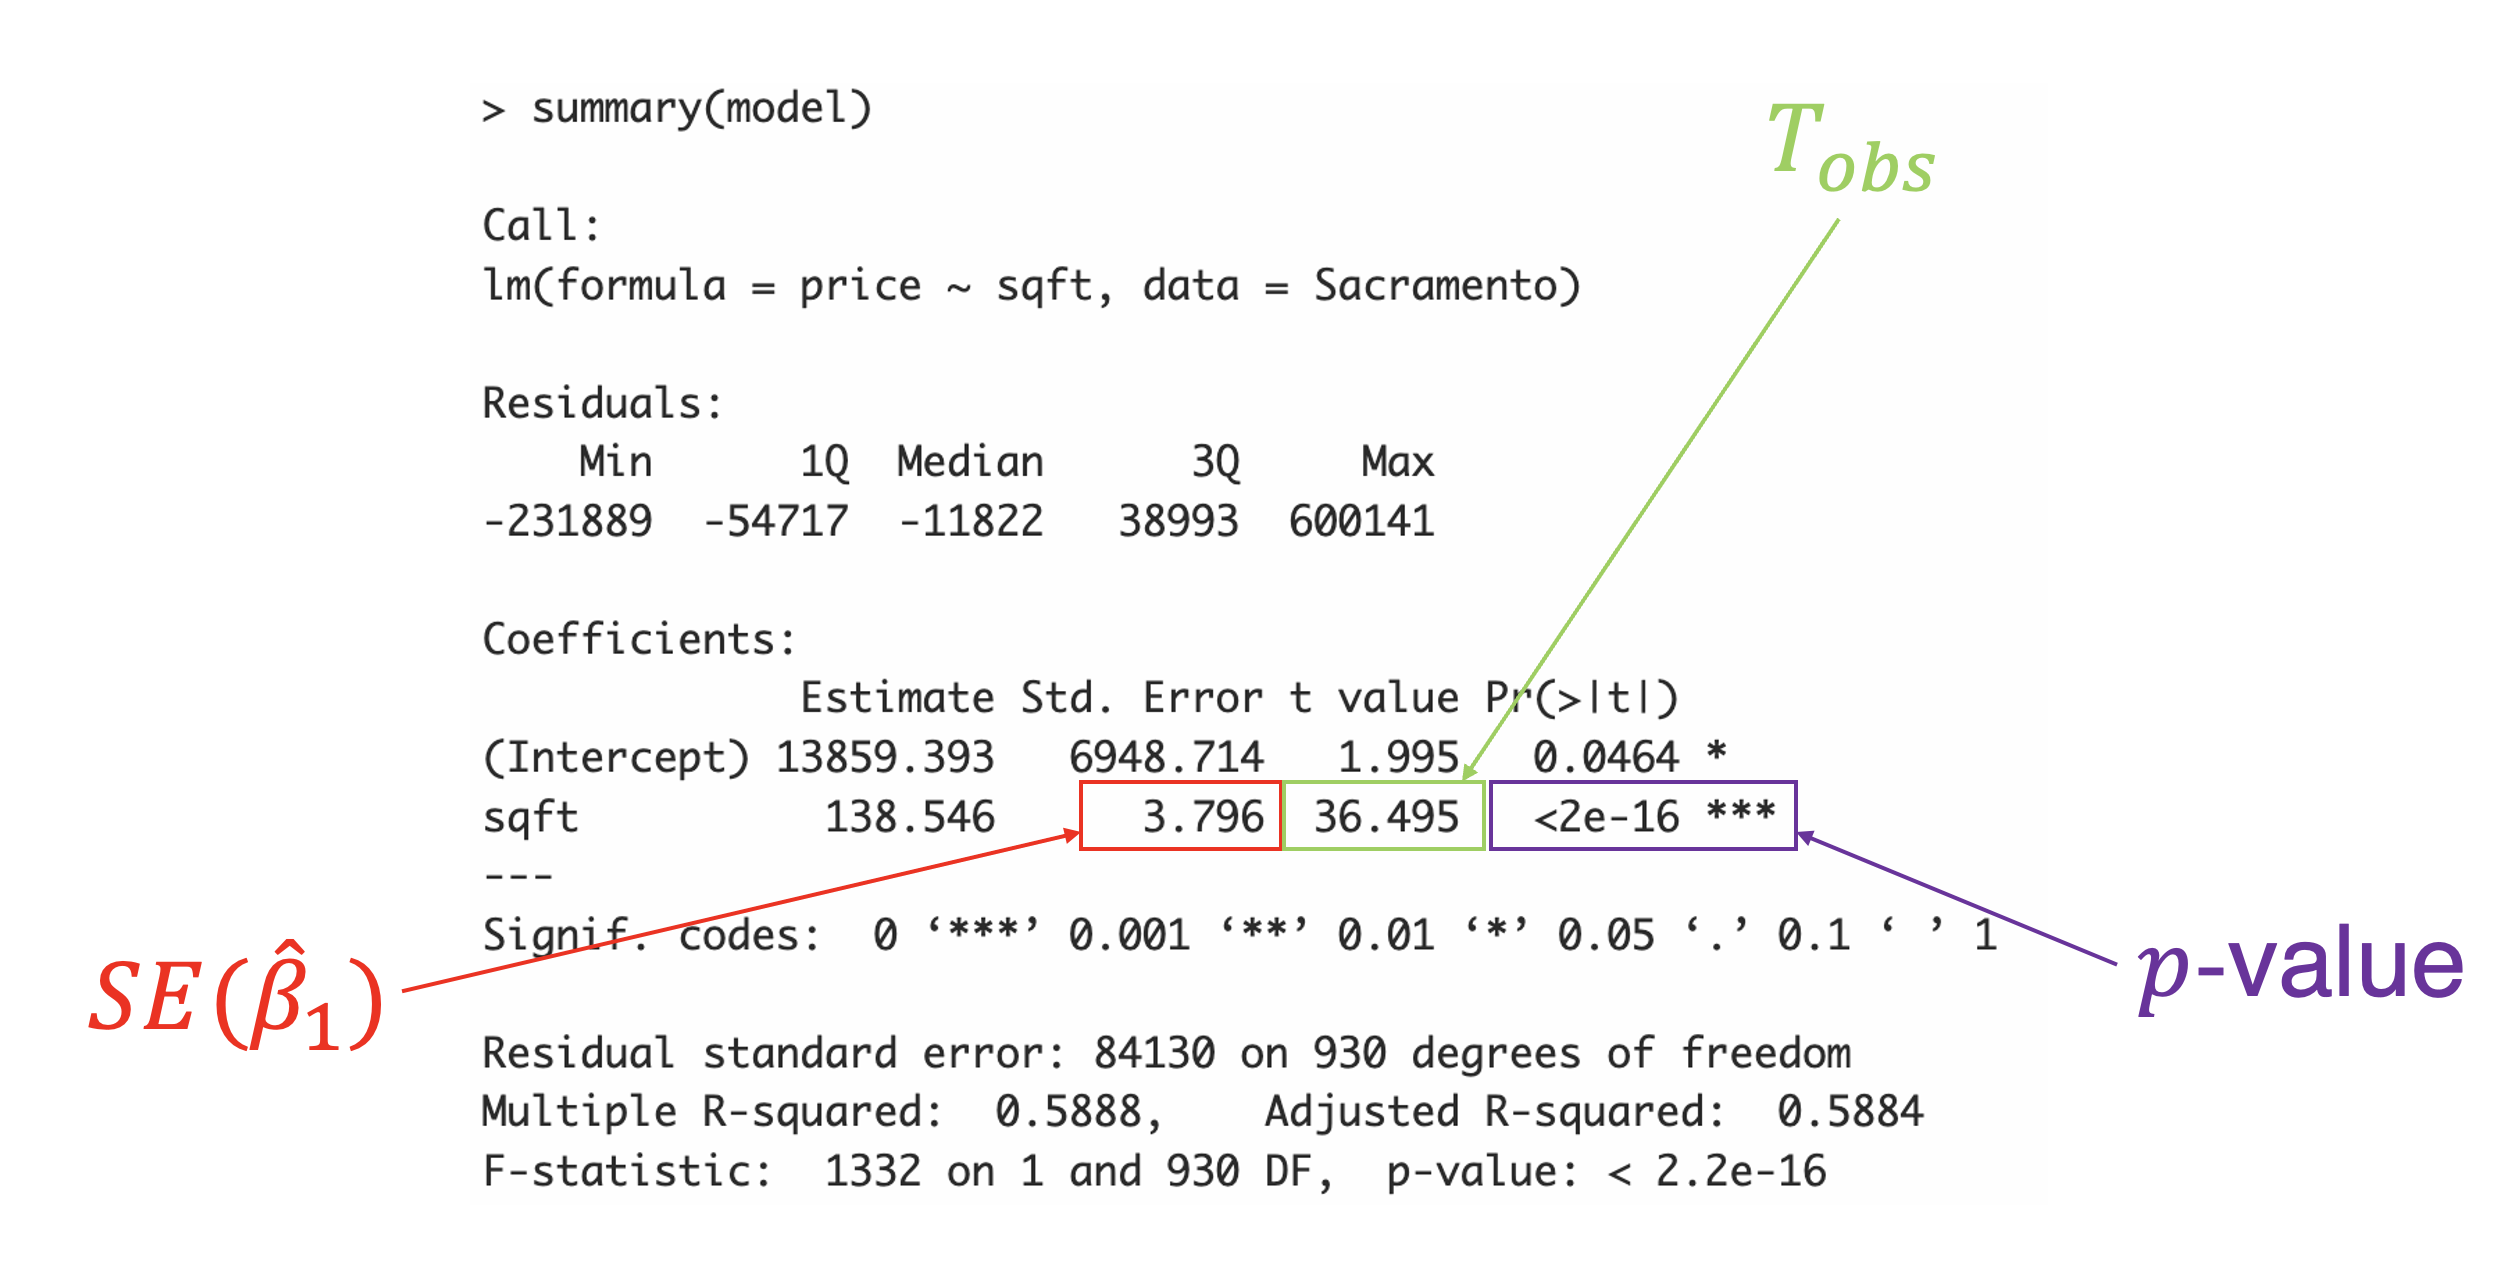
\includegraphics[width=\linewidth]{figures/se_t_p.png}
    \end{center}
\end{frame}

\begin{frame}{Analysis of Variance}
    The analysis of variance for a regression model allows us to determine how much of the variability in the data is captured by the model, i.e., how effective the model is. Begin by defining 
    \begin{equation*}
        SST = \sum_{i=1}^n (Y_i - \bar{Y})^2 \geq 0
    \end{equation*}
    $SST$ is the total sum of squares and represents the total variability in the response.
\end{frame}

\begin{frame}{Total Sum of Squares}
    \begin{center}
        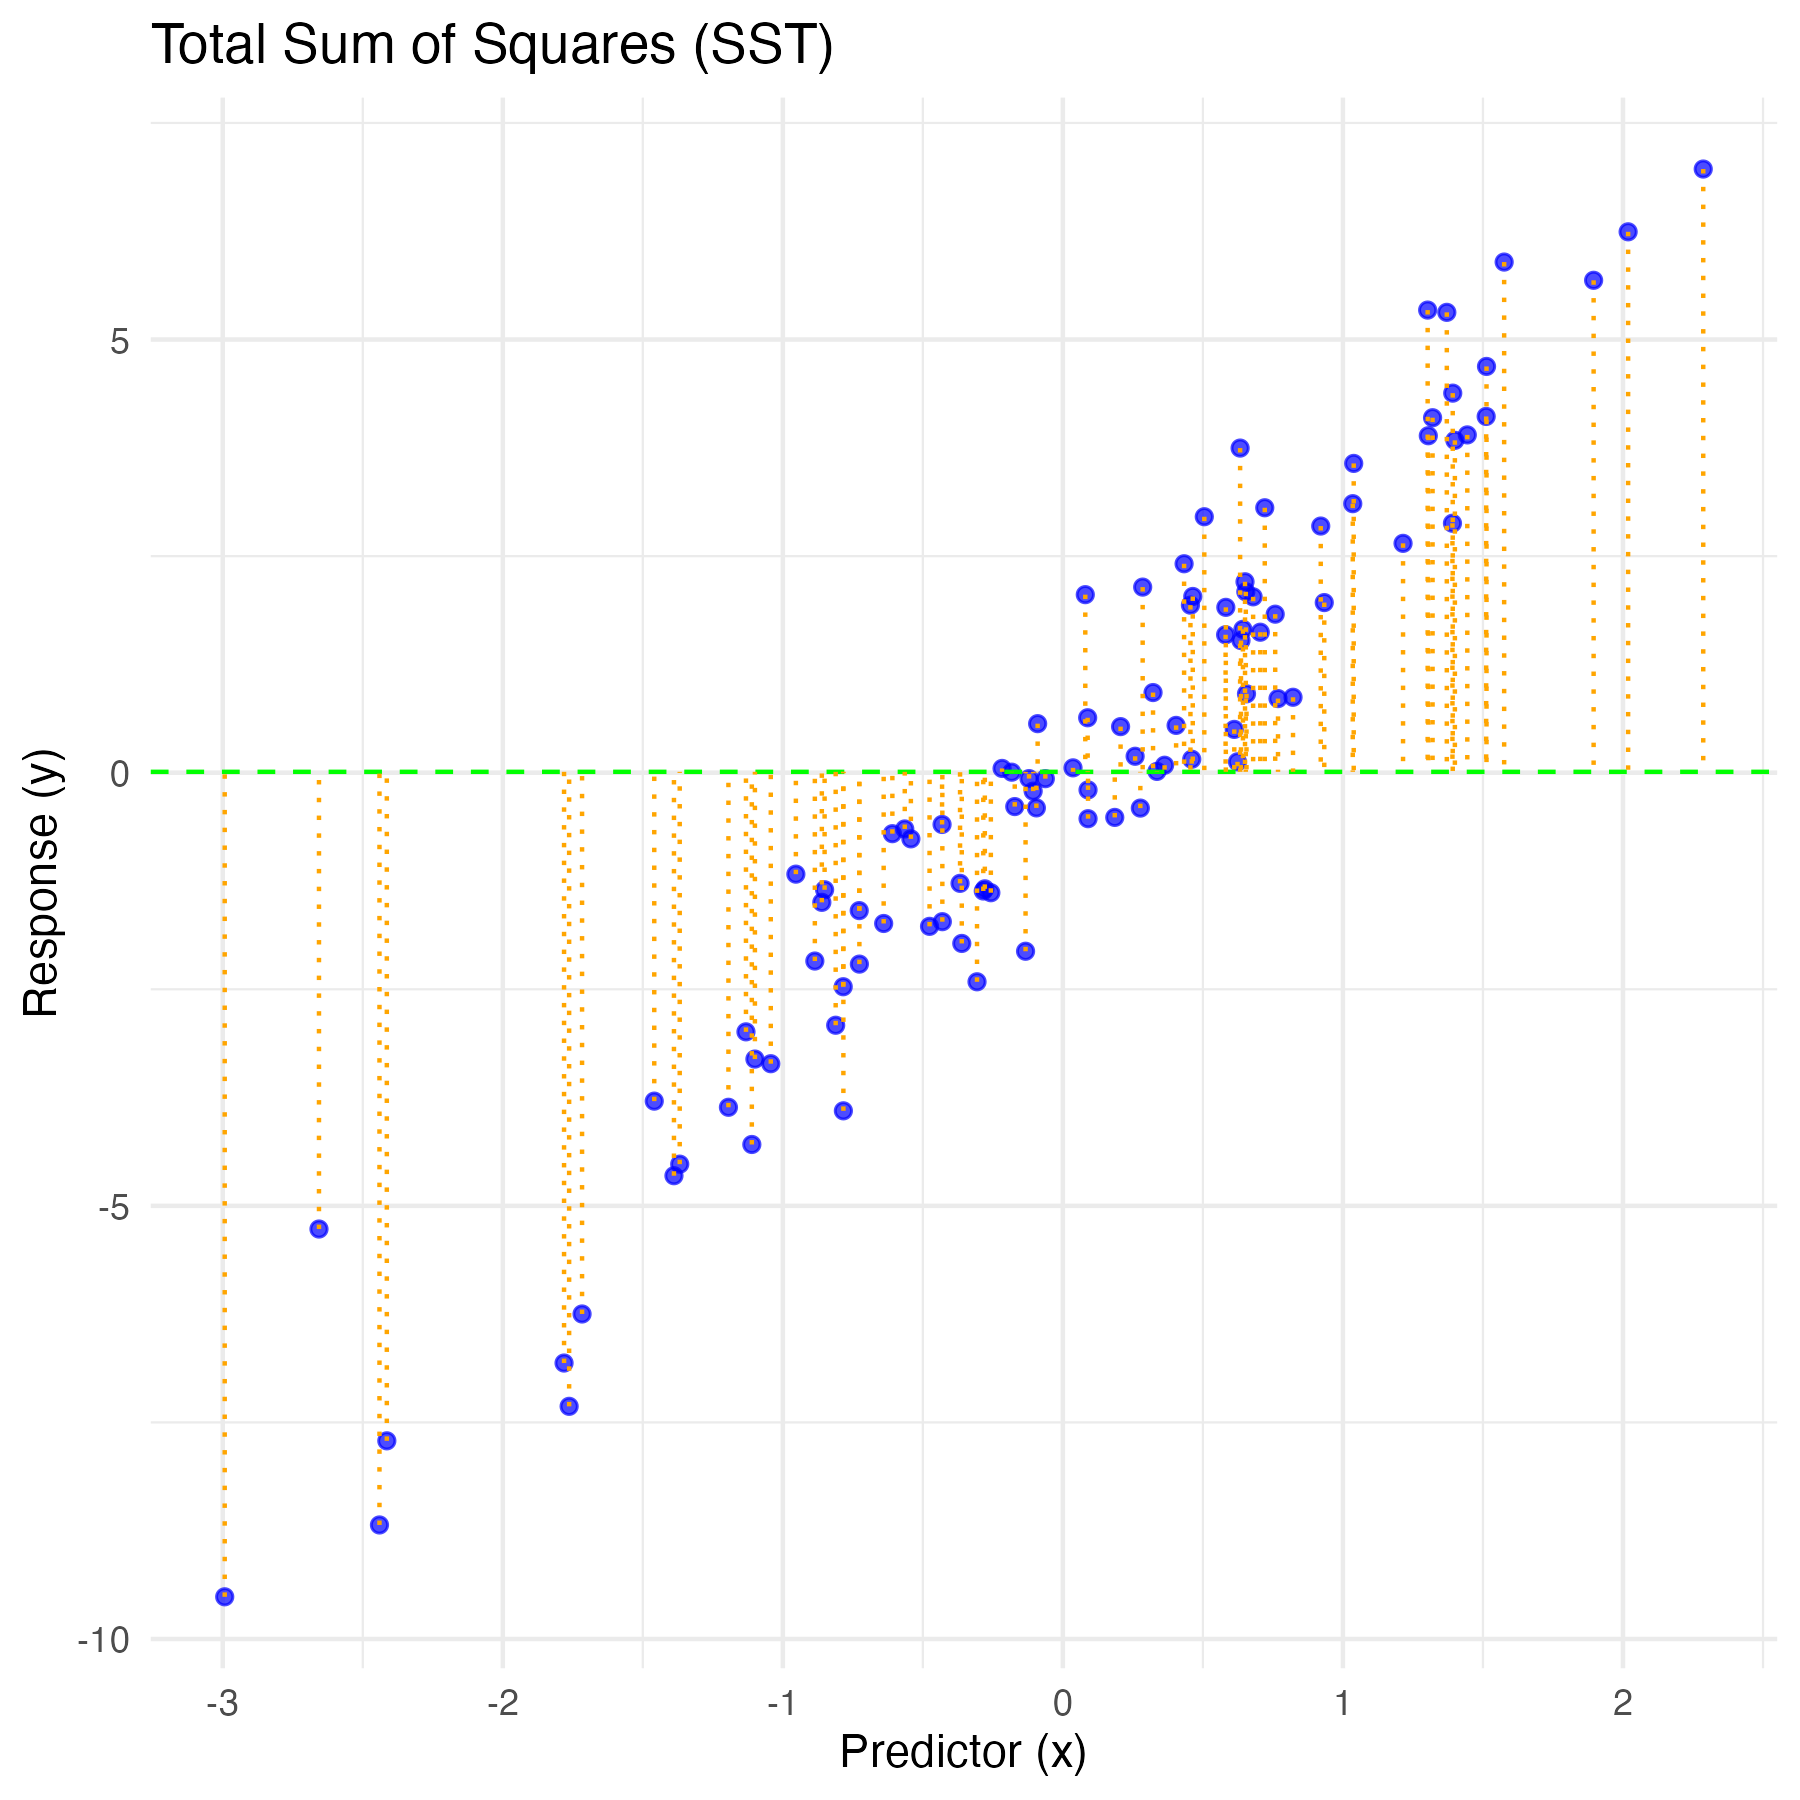
\includegraphics[width=.7\linewidth]{figures/sst.png}
    \end{center}
\end{frame}

\begin{frame}{Analysis of Variance}
    The analysis of variance \textit{decomposes} the total variability into two terms:
    \begin{equation*}
        SST = SSR + SSE
    \end{equation*}
    Therefore, $0 \leq SSR \leq SST$ and $0\leq SSE \leq SST$. 
\end{frame}

\begin{frame}{Analysis of Variance}
    We will determine how effective the model is by determining what proportion of $SST$ is captured by the model. The \textbf{regression} sum of squares is 
    \begin{equation*}
        SSR = \sum_{i=1}^n (\hat{Y}_i - \bar{Y})^2
    \end{equation*}
    \begin{itemize}
        \item $SSR$ is large if fitted values are far from the mean response 
        \item $SSR$ is small if the fitted values are all near the mean response
    \end{itemize}
\end{frame}

\begin{frame}{Regression Sum of Squares (SSR)}
    \begin{columns}
        \begin{column}{0.5\linewidth}
            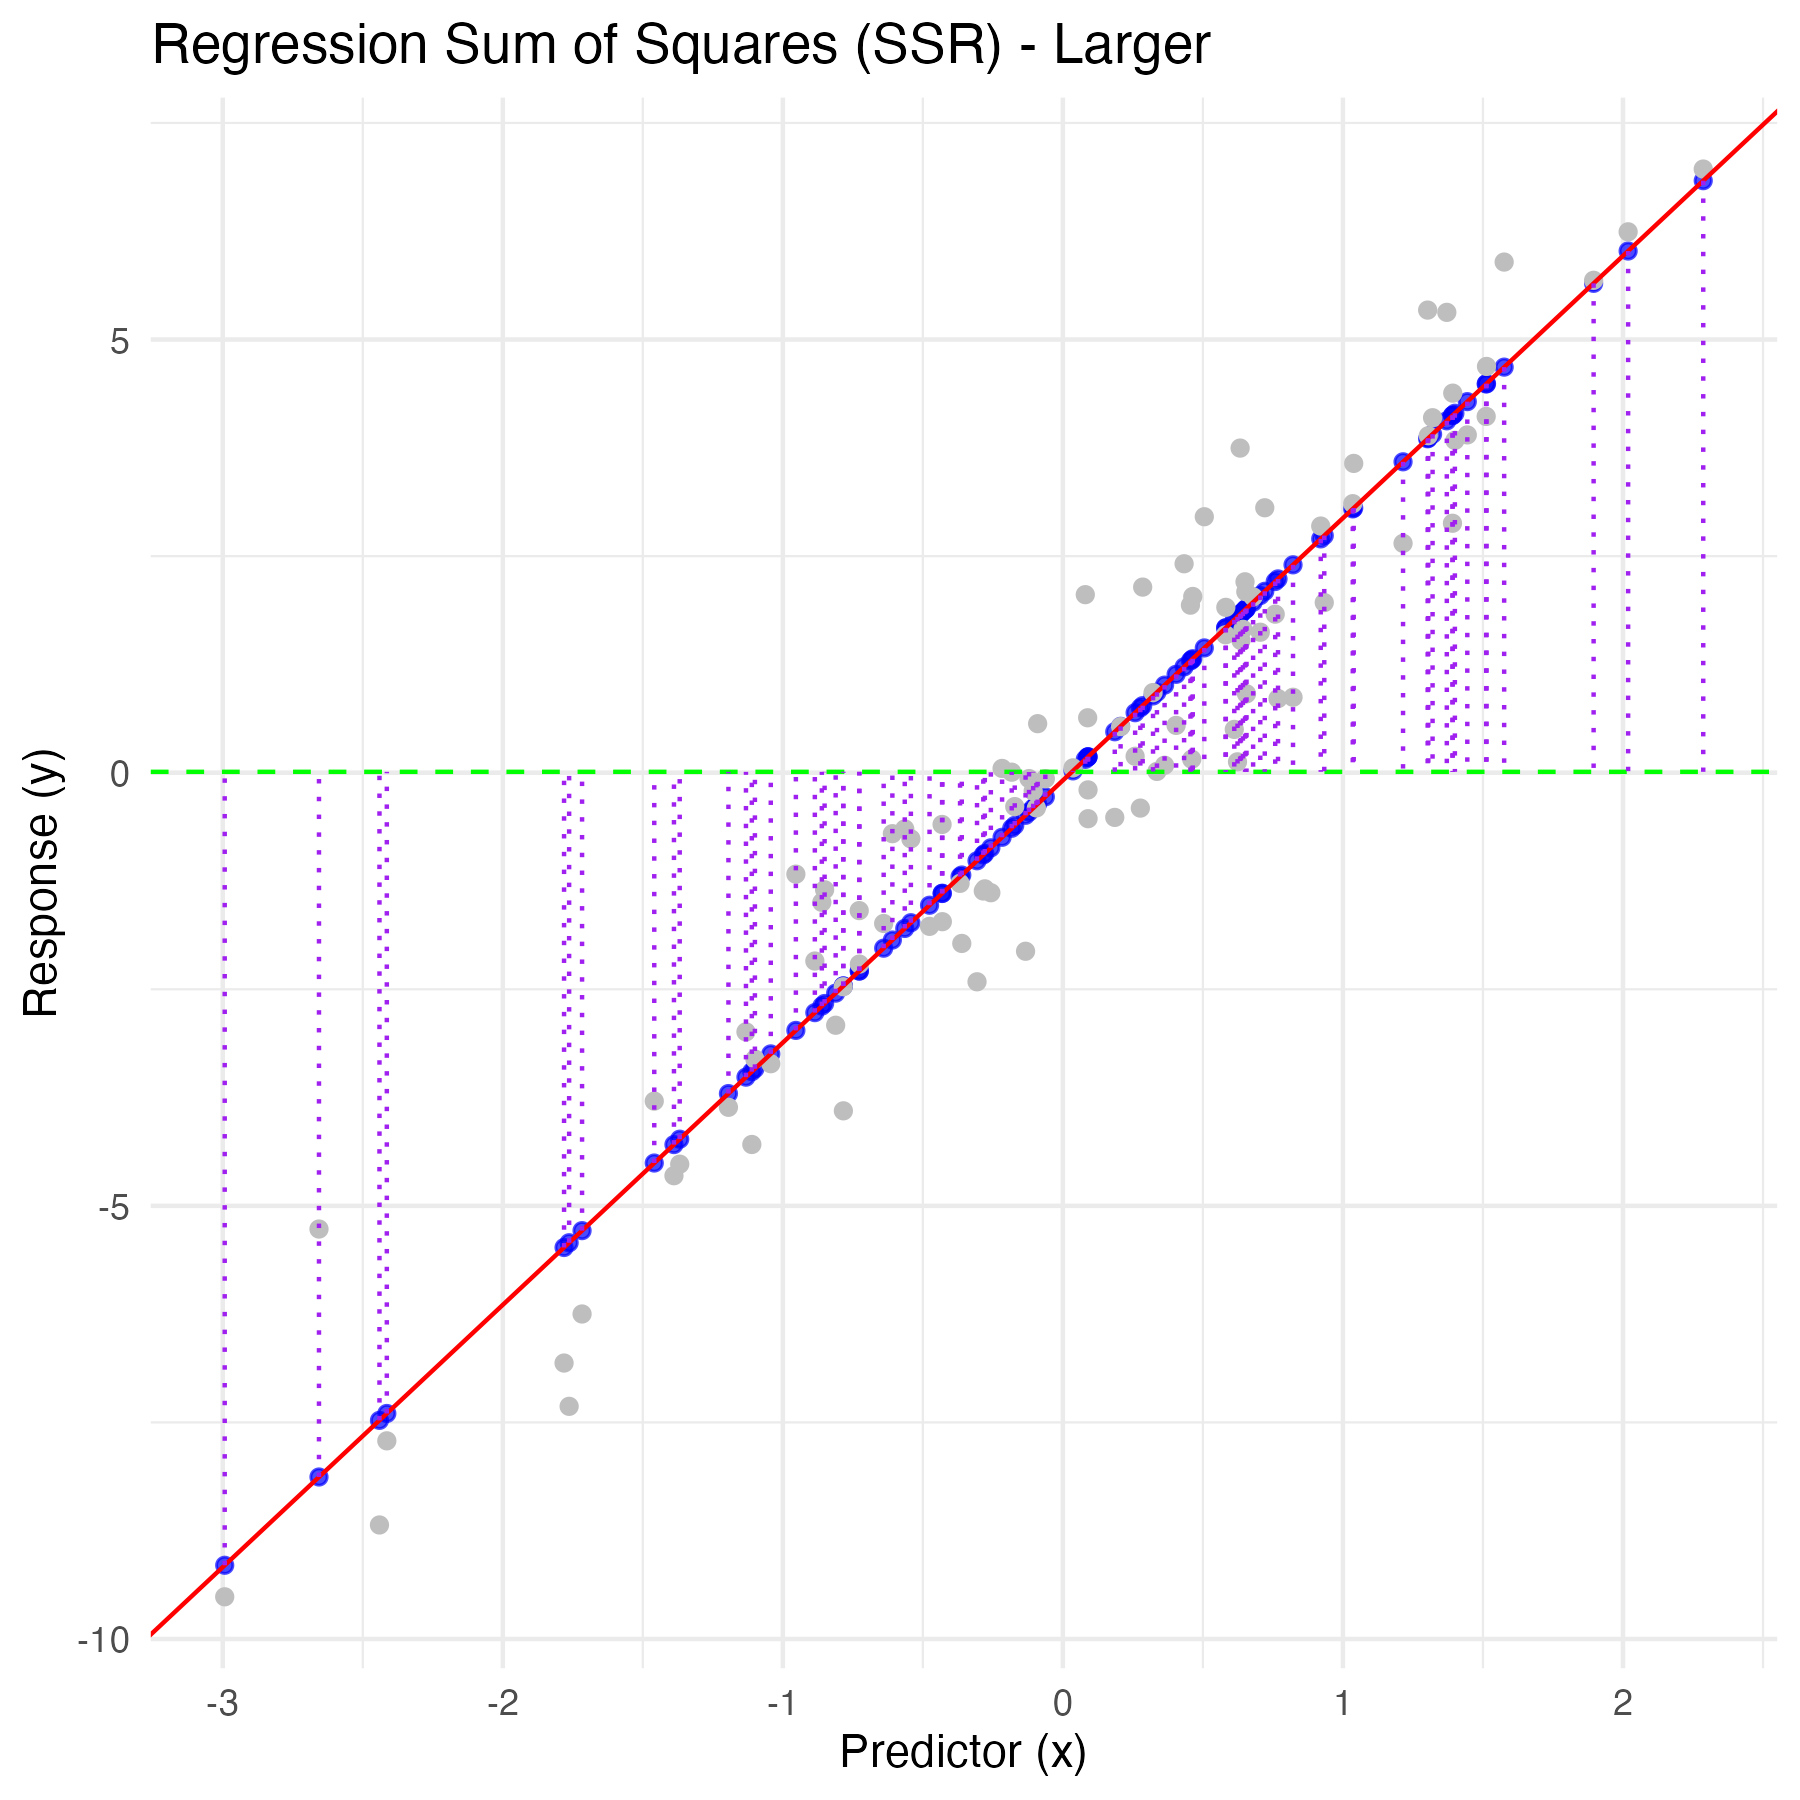
\includegraphics[width=\linewidth]{figures/ssr.png}
        \end{column}
        \begin{column}{0.5\linewidth}
            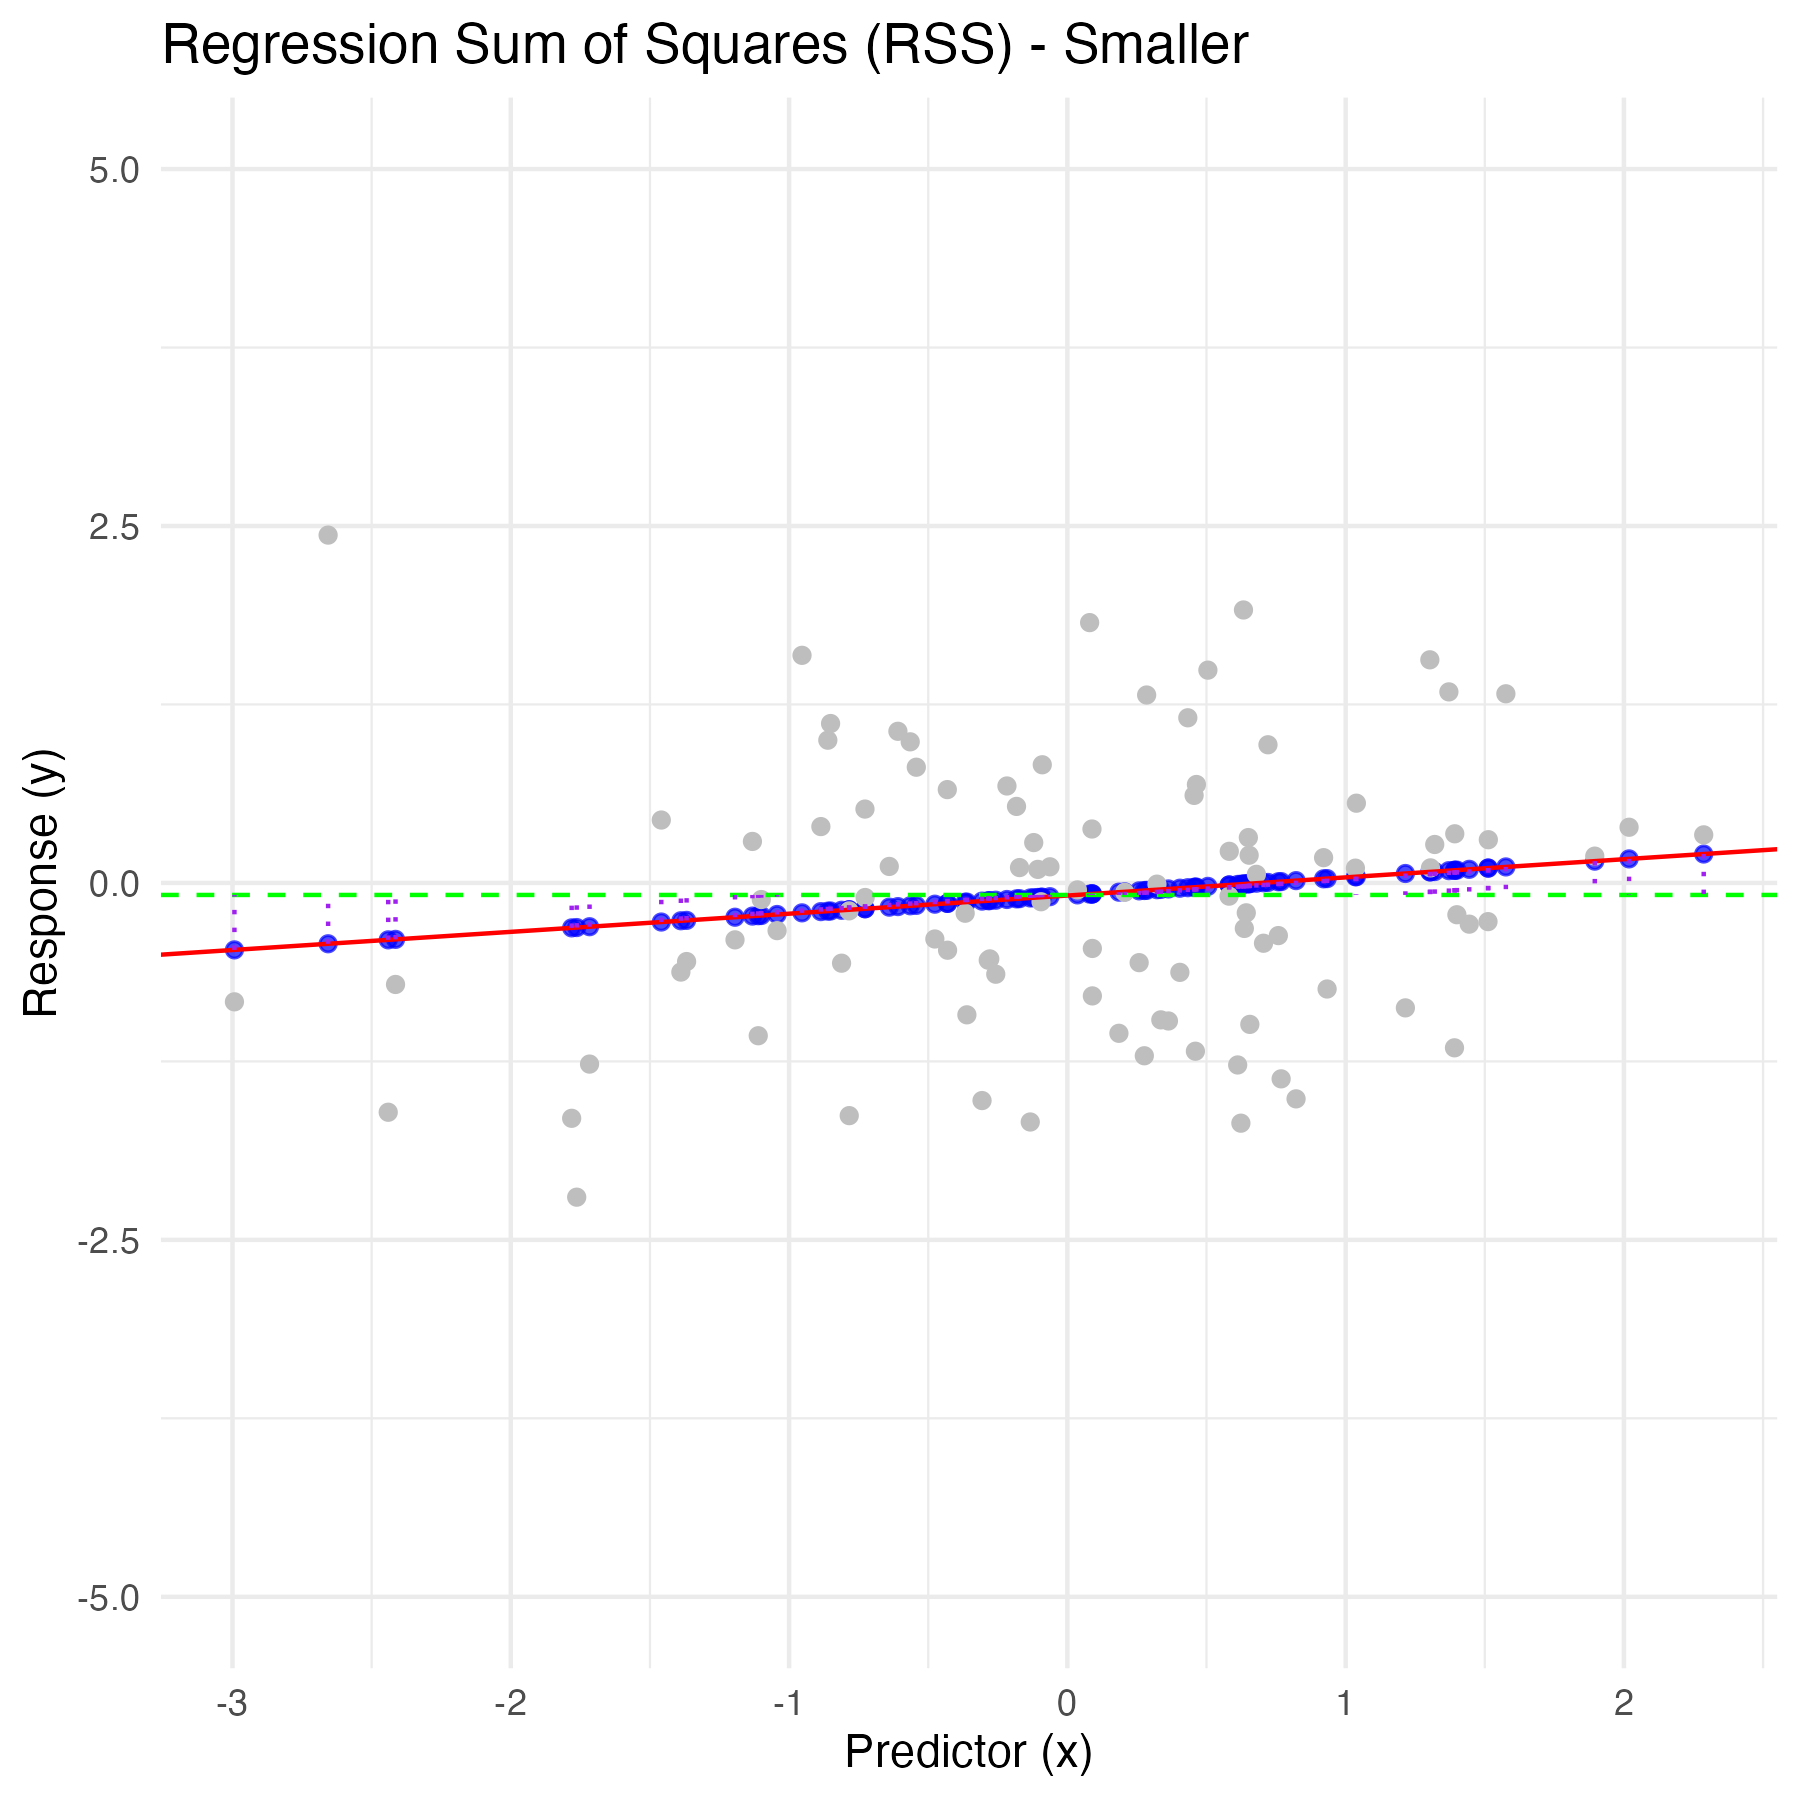
\includegraphics[width=\linewidth]{figures/ssr_small.png}
        \end{column}
    \end{columns}
\end{frame}

\begin{frame}{Residual Sum of Squares}
    We've already seen the residual sum of squares,
    \begin{equation*}
        RSS\ \textrm{or}\ SSE = \sum_{i=1}^n \hat{\varepsilon}_i^2 = \sum_{i=1}^n (Y_i - \hat{Y}_i)^2
    \end{equation*}
    which is also called the sum of squared errors $SSE$.
    \begin{itemize}
        \item Large $RSS$ means lots of scatter around the regression line.
    \end{itemize}
\end{frame}

\begin{frame}{Residual Sum of Squares (SSE)}
    \begin{columns}
        \begin{column}{0.5\linewidth}
            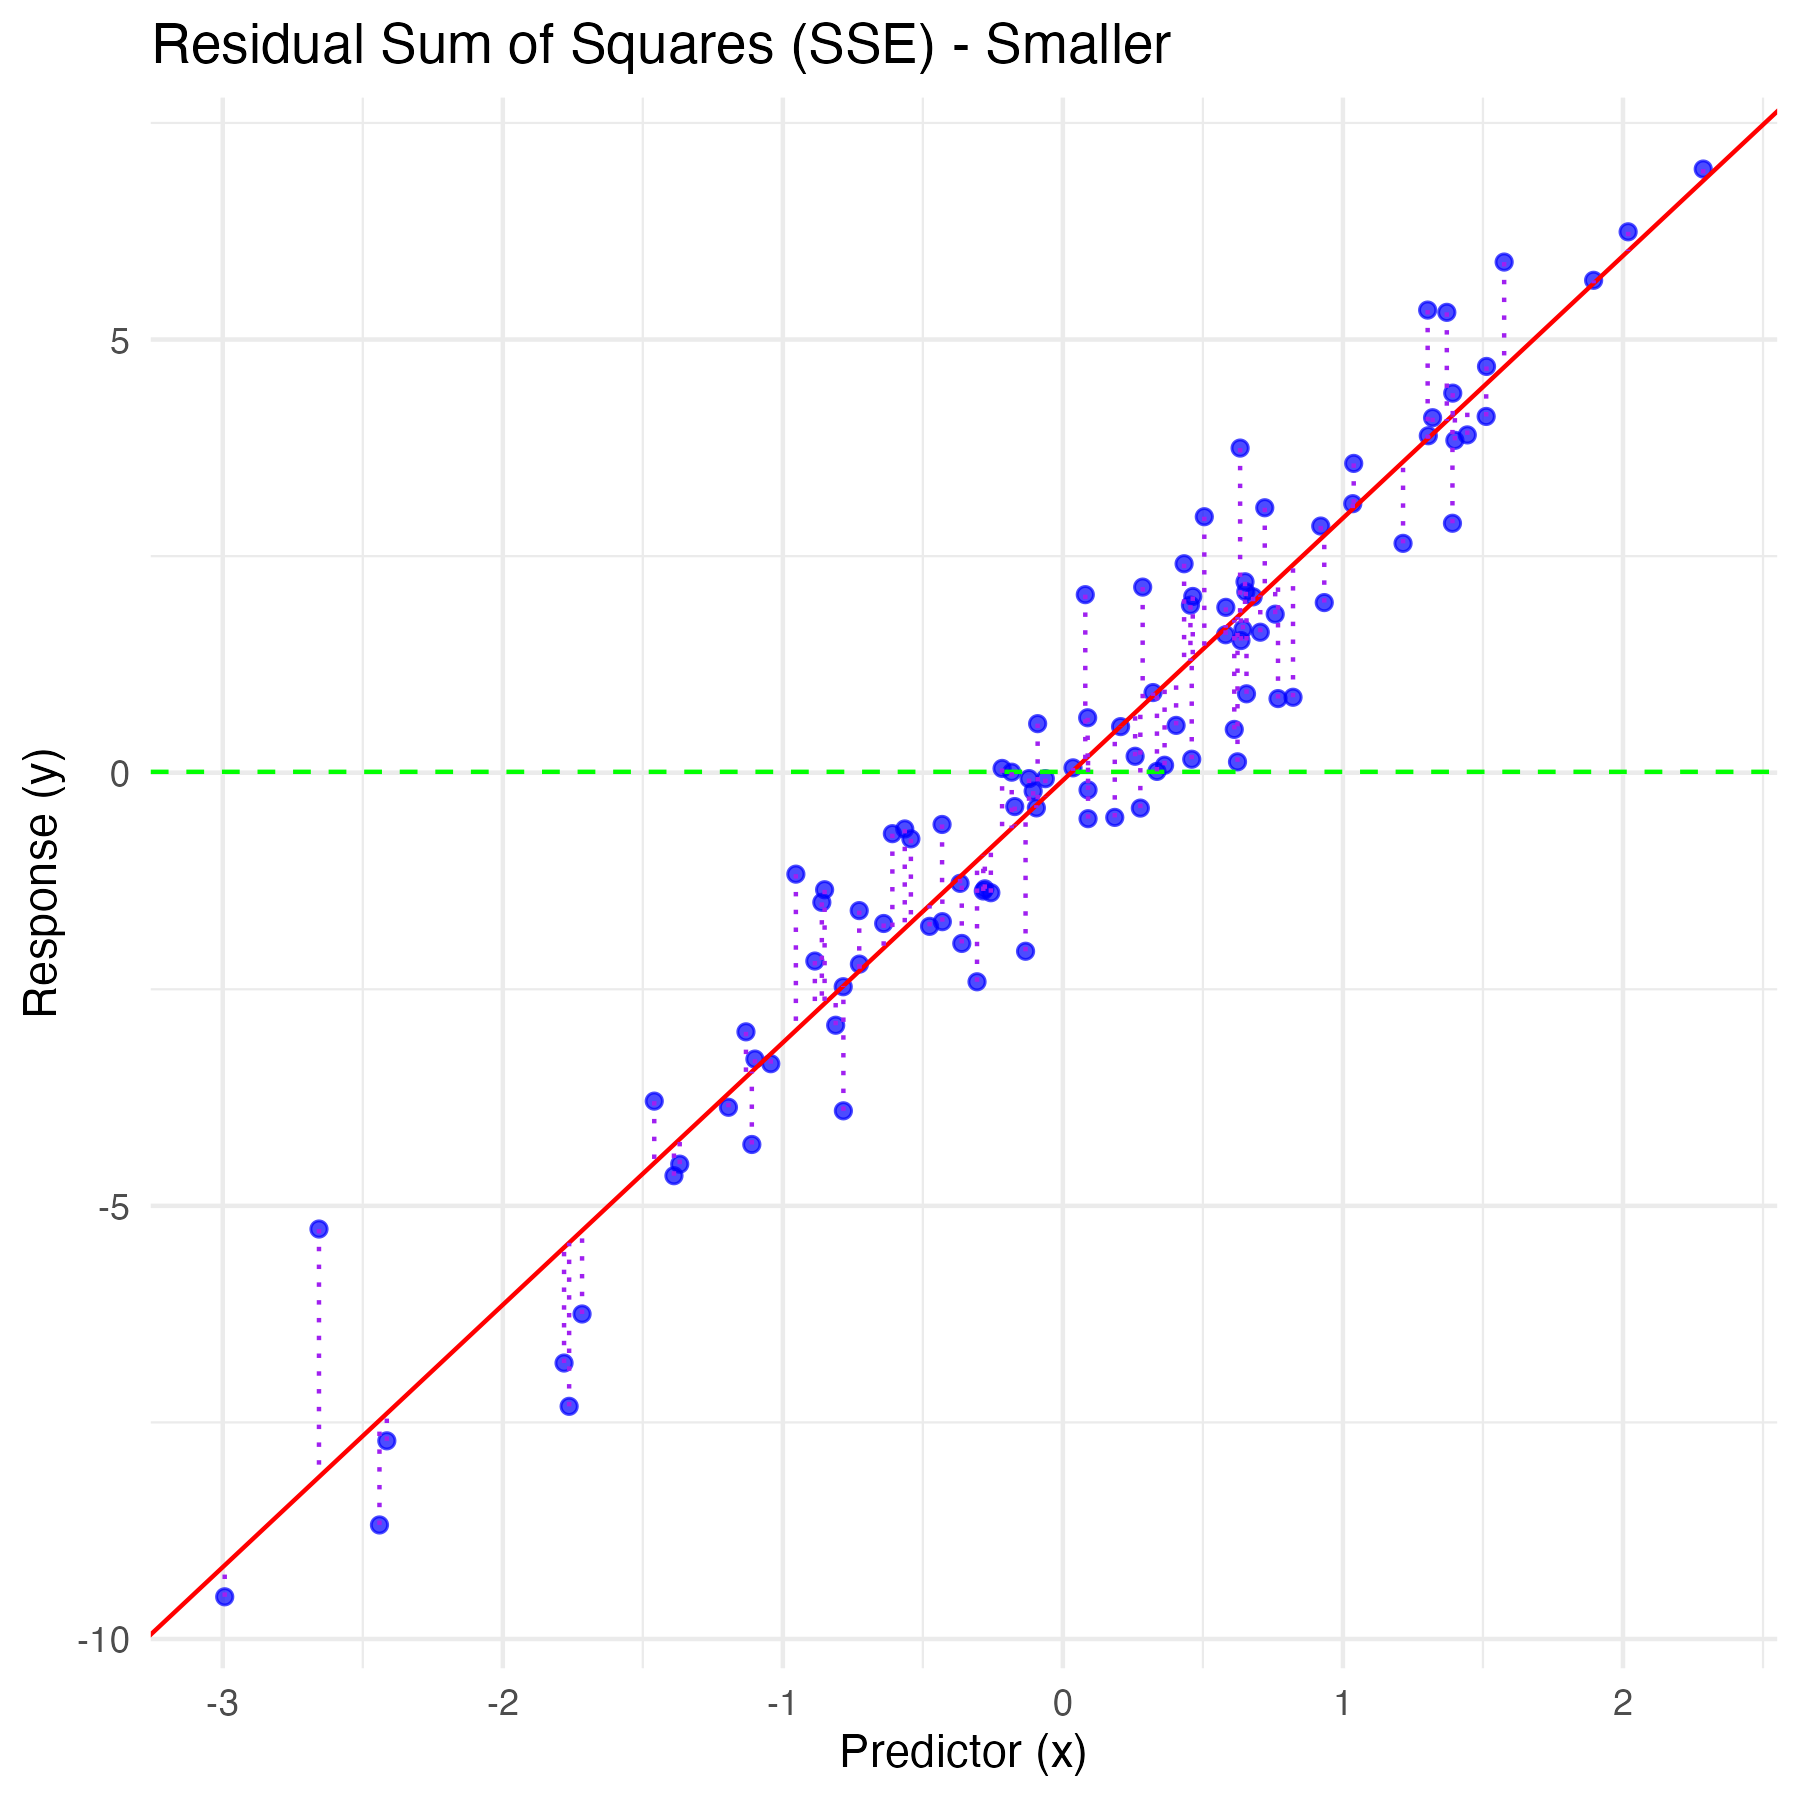
\includegraphics[width=\linewidth]{figures/sse.png}
        \end{column}
        \begin{column}{0.5\linewidth}
            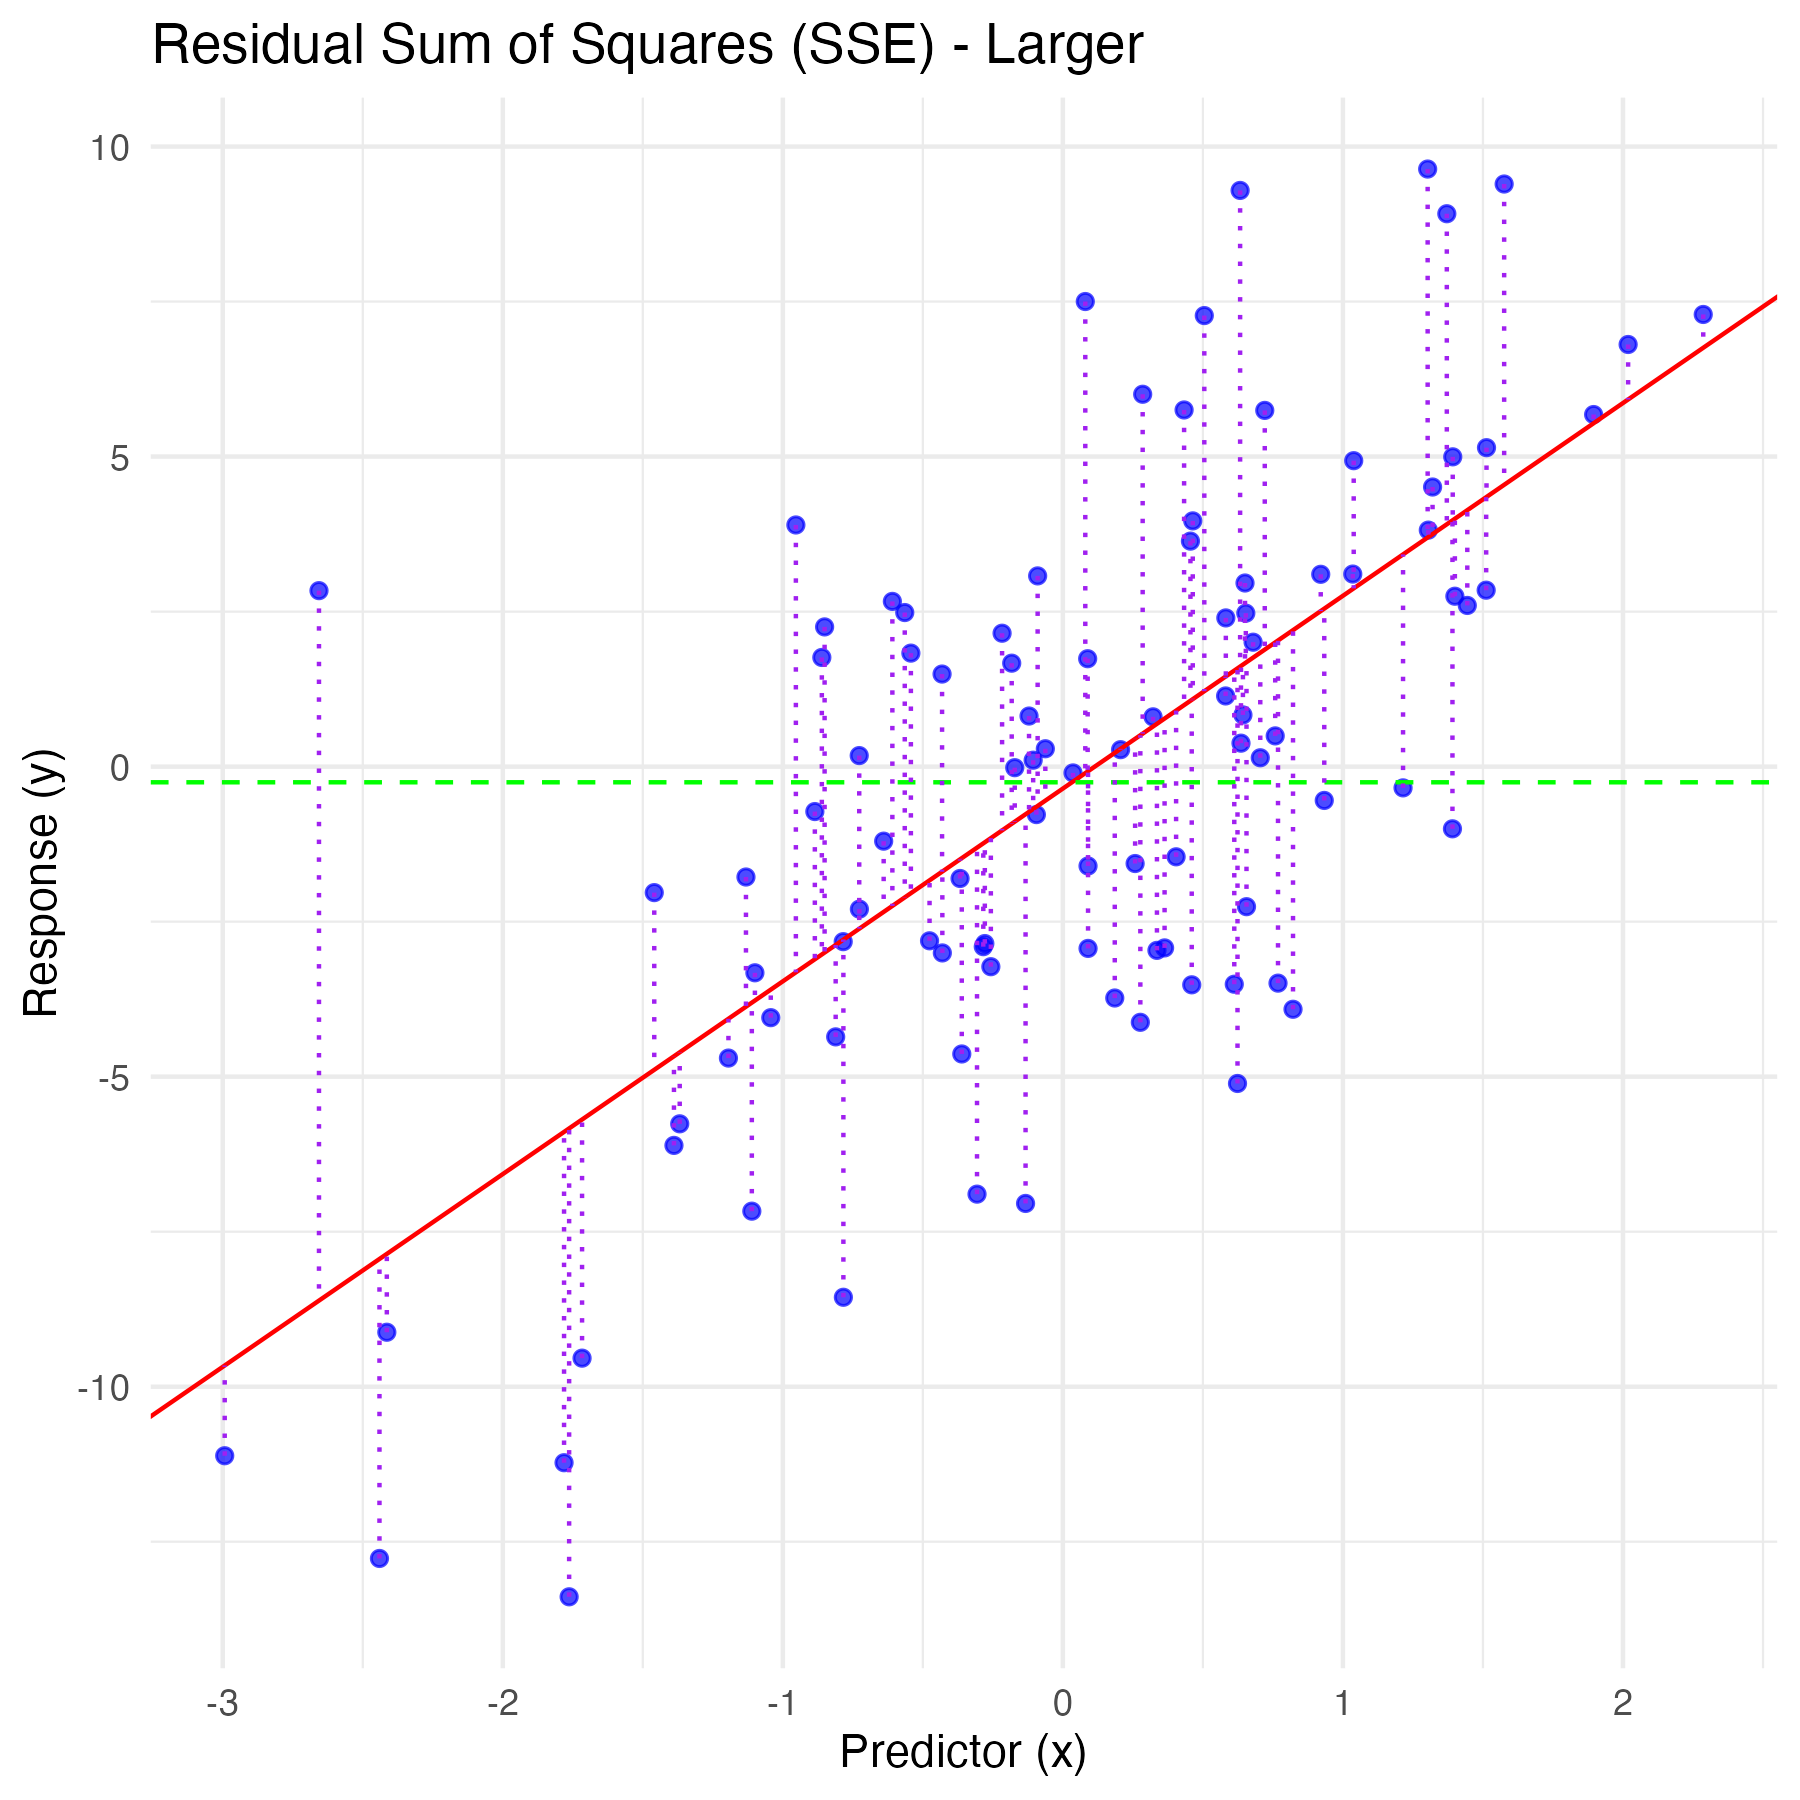
\includegraphics[width=\linewidth]{figures/sse_larger.png}
        \end{column}
    \end{columns}
\end{frame}

\begin{frame}{Coefficient of Determination $R^2$}
    The \textbf{coefficient of determination} is 
    \begin{equation*}
        R^2 = \frac{SSR}{SST} = 1 - \frac{SSE}{SSR}
    \end{equation*}
    \begin{itemize}
        \item $R^2$ is the square of the correlation between $X$ and $Y$.
        \item $0\leq R^2\leq 1$.
        \item $R^2$ is interpreted as the percentage of variability in $Y$ captured by the regression model.
    \end{itemize}
\end{frame}

\begin{frame}{Reading \texttt{R} Output}
    \begin{center}
        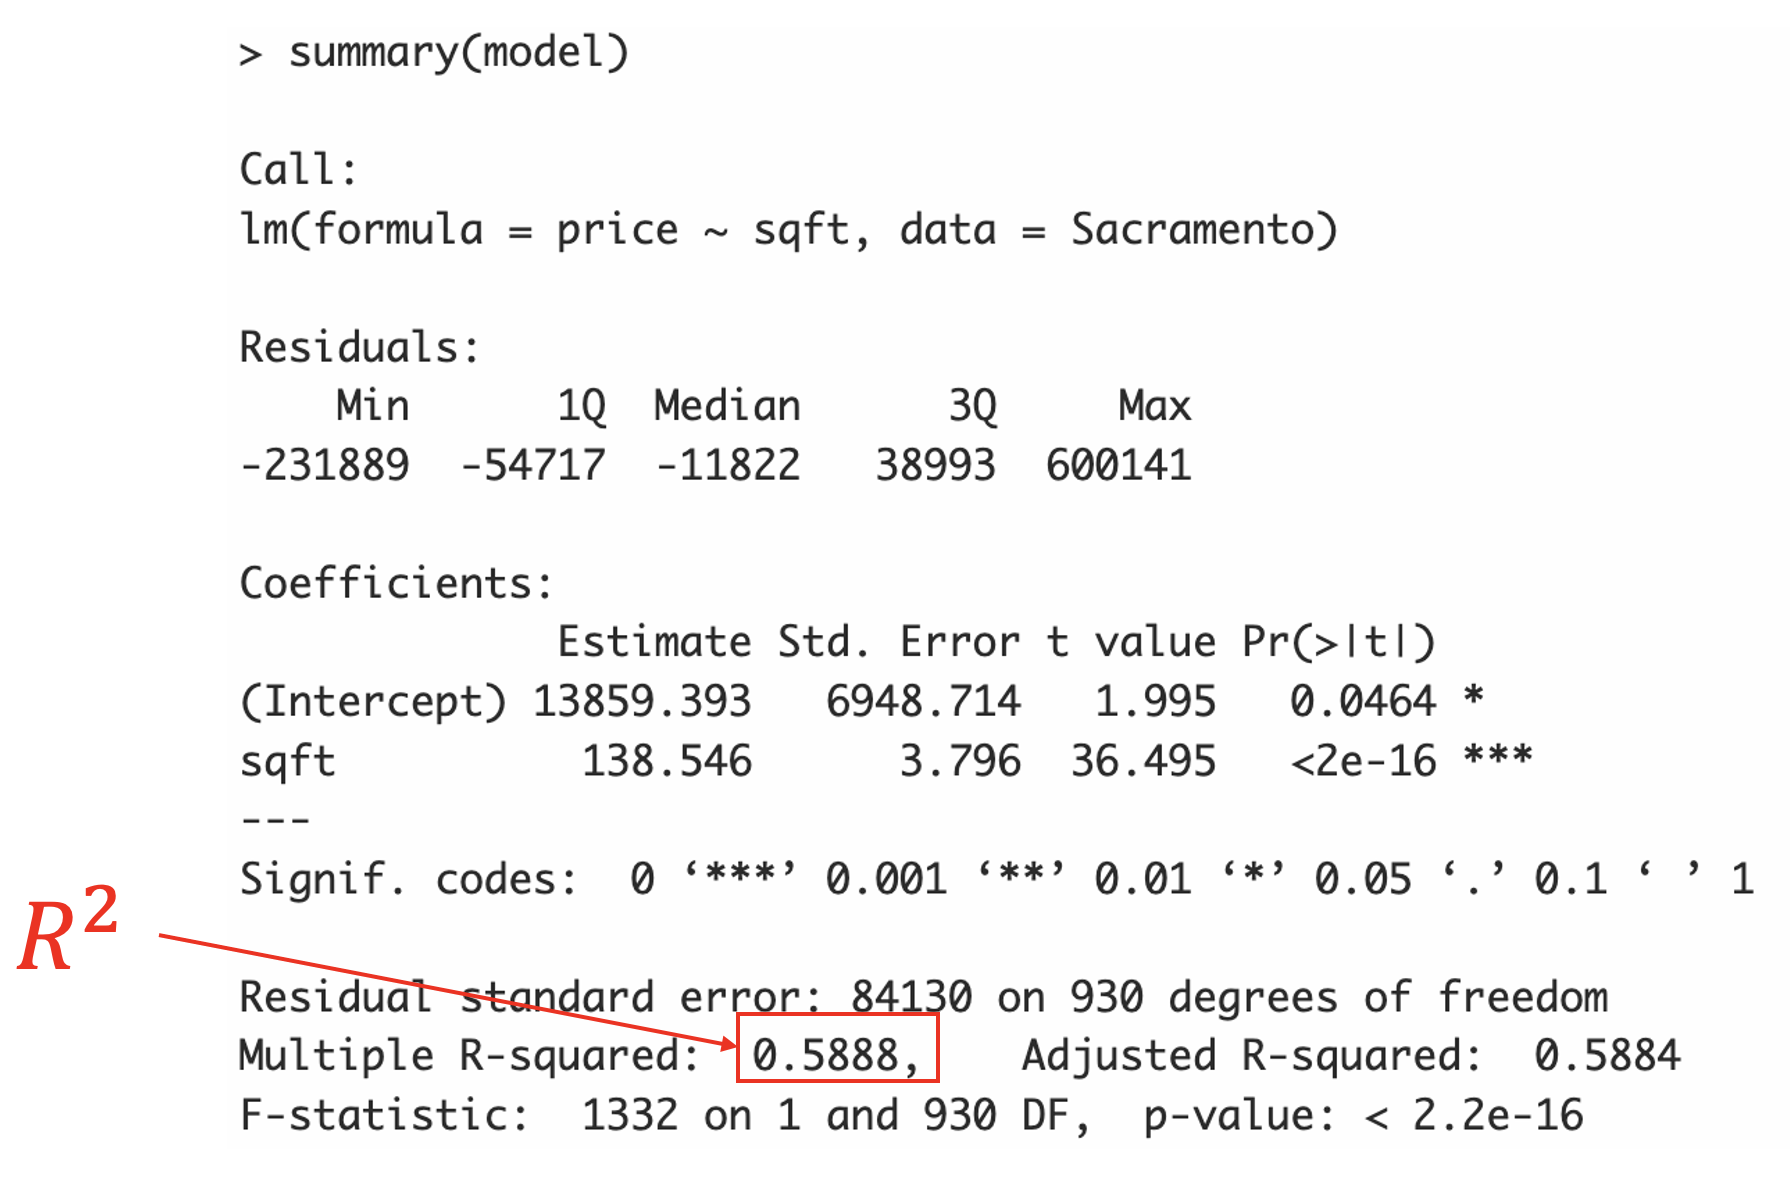
\includegraphics[width=\linewidth]{figures/r-squared.png}
    \end{center}
\end{frame}

\begin{frame}{Prediction}
    With the fitted model, we may want to predict $\hat{Y}^* = \mathbb{E}[Y | X^**]$ given a new value of $X^*$. 

    \vspace*{1em}

    For the housing data, we predict the \textit{average} price given the square footage of a new house by
    \begin{equation*}
        \textrm{Price} = \hat{\beta}_0 + \hat{\beta}_1 \times \textrm{Square Footage}
    \end{equation*}

    We predict the \textit{average} price of houses with a square footage of 2,000 by 
    \begin{equation*}
        13859.393 + 138.546 \times 2000 = \$290,951.4
    \end{equation*}
\end{frame}

\begin{frame}{Confidence Interval for Regression Line}
    A $(1-\alpha)\times 100$\% confidence interval for $\hat{Y}^* = \mathbb{E}[Y | X^*]$ using the least squares estimates $\hat{\beta}_0$ and $\hat{\beta}_1$ is 
    \begin{equation*}
        \hat{Y}^* \pm t^*_{\alpha/2, n-2} \hat{\sigma}\times \sqrt{\frac{1}{n} + \frac{(X^* - \bar{X})^2}{SXX}}
    \end{equation*}
    Sources of uncertainty:
    \begin{itemize}
        \item Regression parameters: $\hat{\beta}_0$ and $\hat{\beta}_1$ and 
        \item Error variance $\hat{\sigma}^2$. 
    \end{itemize}
\end{frame}

\begin{frame}{Prediction Intervals}
    The previous interval was a confidence interval for the average value $\hat{Y}^* = \mathbb{E}[Y | X^*]$ given a value of the predictor $X^*$.  
    \begin{itemize}[<+->]
        \item $\hat{Y}^* = \mathbb{E}[Y | X^*]$ is what we expect $Y$ to be in long run when $X = X^*$.
        \item $\hat{Y}^* = \mathbb{E}[Y | X^*]$ is \textit{fixed} but unknown.
        \item Values of $Y$ when $X = X^*$ can vary around $\hat{Y}^*$.
        \item Confidence intervals are for unknown parameters (e.g., $\hat{Y}^* = \mathbb{E}[Y | X^*]$).
        \item Prediction intervals are for random variables (e.g., $Y^*$) and will be wider than confidence intervals.
    \end{itemize}
\end{frame}

\begin{frame}{Prediction Intervals}
    A $(1-\alpha)\times 100$\% prediction interval for the actual value $Y^*$ when $X = X^*$ is 
    \begin{equation*}
        \hat{Y}^* \pm t^*_{\alpha/2, n-2} \hat{\sigma} \times \sqrt{{\color{red} 1} + \frac{1}{n} + \frac{(X^* - \bar{X})^2}{SXX}}
    \end{equation*}
    where $\hat{Y}^* = \hat{\beta}_0 + \hat{\beta}_1 X^*$. Sources of uncertainty/variability:
    \begin{itemize}
        \item Regression parameters: $\hat{\beta}_0$ and $\hat{\beta}_1$ and 
        \item Error variance $\hat{\sigma}^2$. 
        \item {\color{red} Random fluctuation of actual values around the regression line.}
    \end{itemize}
\end{frame}

\begin{frame}{Intervals in \texttt{R}}
    Use the \texttt{predict} function\footnote{See R notes on Canvas}. \par 
    \vspace*{1em}
    \footnotesize

    \texttt{> model <- lm(price $\sim$ sqft, data = Sacramento)} \par 
    \texttt{> predict(model, 
    newdata = data.frame(sqft = 2000), 
    interval = \textbf{"confidence"}, 
    level = 0.95)} \par 
    \texttt{\quad\quad\quad\quad fit\quad\quad\quad\quad lwr\quad\quad\quad upr}\par 
    \texttt{1 290952.3 285043.1 296861.5}\par 
    \texttt{> predict(model, 
    newdata = data.frame(sqft = 2000), 
    interval = \textbf{"prediction"}, 
    level = 0.95)} \par 
    \texttt{\quad\quad\quad\quad fit\quad\quad\quad\quad lwr\quad\quad\quad upr}\par 
    \texttt{1 290952.3 125748.3 456156.3}
\end{frame}

\end{document}